\chapter{Machine learning}

\section{Nearest neighbor classification}

\subsection{Digit recognition}

Countless pieces of mail pass through the postal service daily. A key step in handling
them efficiently is {\it automatically scanning and parsing their destination zipcodes}.
Each zipcode can be segmented into five (or sometimes nine) digits. Here is a smattering
of them:

\begin{center}
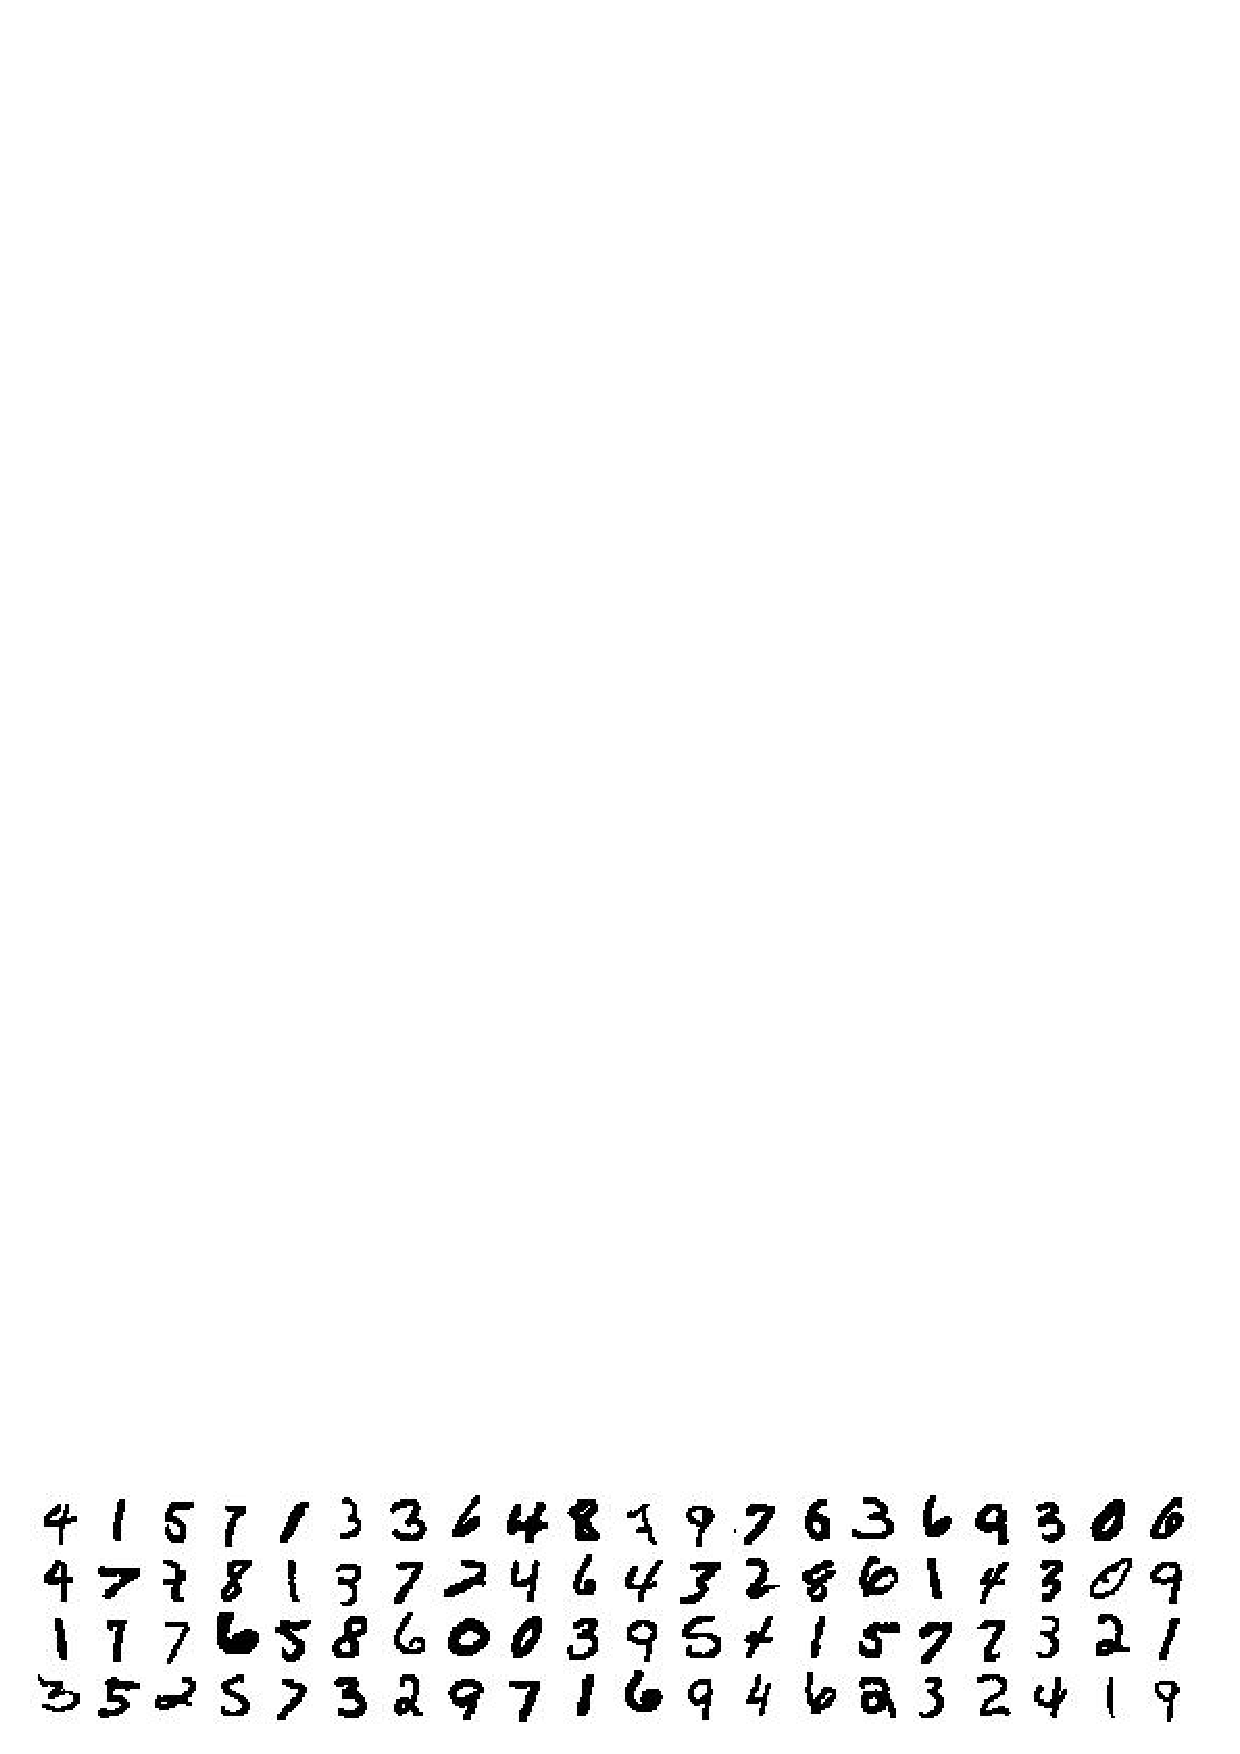
\includegraphics[width=6in]{figs/mnist.pdf}
\end{center}

\noindent
How can each such image be mapped to the corresponding digit? One approach is to
use {\it hand-coded rules}. This would involve two steps:
\begin{itemize}
\item Write subroutine to identify key features (such as loops) of an image.
\item Write a bunch of rules, like ``if there's a loop then it's not a 1,3,5 or 7''.
\end{itemize}
Both steps are problematic. As you can see from the examples above, real handwritten
digits are rife with deviations from ideal script, such as almost-loops. These 
variations can easily trip up a set of rigid rules. A much better idea is to 
{\it learn a classifier automatically from data}.

\subsection{The input space and the label space}

We want to create a classifier that takes an image $x$ and outputs a label $y$.
What are the spaces $\X$ and $\Y$ from which these images and labels are drawn?

The Post Office has made available a {\it training set} of $60{,}000$ digit-images. 
Each of these is a $28 \times 28$ greyscale image of a single digit. We can represent 
an image $x$ by a vector of 784 coordinates, one per pixel. The input space is then
$\X = \R^{784}$. The label space is, naturally, $\Y = \{0,1,\ldots, 9\}$. Thus the 
classifier we seek is a function $f: \X \rightarrow \Y$.

The training set can be written as $(x_1, y_1), \ldots, (x_n,y_n)$ where $n = 60{,}000$
and each $x_i \in \X$, $y_i \in \Y$. How can we use this data to find a good classifier
$f$?

\subsection{A nearest neighbor classifier}

Here's a simple classifier: for any image $x$, the label $f(x)$ is given by the 
following procedure.
\begin{itemize}
\item Find the $x_i$ that is closest to $x$ (out of $x_1, \ldots, x_n$).
\item Return $y_i$.
\end{itemize}
What is meant by ``closest to''? Well, we can use any notion of distance. One
natural option is just Euclidean distance. For two dimensional vectors 
$a = (a_1, a_2)$ and $b = (b_1, b_2)$, the Euclidean distance is given by the
familiar formula
$$ \|a - b\| \ = \ \sqrt{(a_1 - b_1)^2 + (a_2 - b_2)^2} .$$
A similar formula applies in higher dimensions. For $a,b \in \R^d$, we have
$$ \|a - b\| \ = \ \sqrt{\sum_{i=1}^d (a_i- b_i)^2} .$$

How good is this classifier? Is it always correct? Well, it is certainly
has zero error on the training set: that is, $f(x_i) = y_i$ for training 
points $(x_i, y_i)$. But $f$ might not be correct for other images $x$. 
How can we assess its accuracy?

To this end, the Post Office has also provided a separate {\it test set} of
different images and their labels. Any classifier can be tried out on this
test set to see what fraction of images it gets correct. The performance on
this test set is then a good indication of the performance of the classifier
in practice (using the standard theory of sampling). It turns out that
the classifier we have just constructed has an error rate of $23\%$ on the
test set.

Randomly guessing a label would have an error rate of $90\%$, so $23\%$ isn't 
too shabby, but it is certainly not good enough for the Post Office's purposes. 
How can we do better?

\subsection{Two improvements}

Euclidean distance is not really an ideal distance measure between images.
Consider two images that are identical, except that one is shifted slightly
to the right, or is rotated slightly, or is slightly thicker. The Euclidean
distance between these images will be substantial. It would be a lot more
sensible to compute the distance between two images $x$ and $x'$ as follows:
\begin{itemize}
\item First maximally ``align'' the two images by translating and rotating them.
\item Then compute Euclidean distance.
\end{itemize}

A further improvement is obtained by looking not just at the nearest neighbor
of $x$, but at the $k$ nearest neighbors (for some small value of $k$ like $7$),
and returning the most common label amongst these neighbors.

When these two changes are made, the error of the classifier on the test set 
drops below $1\%$.

\subsection{The computational complexity of finding the nearest neighbor}

Suppose points $x_1, \ldots, x_n$ lie in $\R^d$. How does one find the nearest
neighbor of a new point $x$? Here's the brute-force method:
\begin{itemize}
\item Compute all distances $\|x_i - x\|$.
\item Pick the $x_i$ for which this is smallest.
\end{itemize}
This algorithm takes time $O(n)$, which is prohibitive when $n$ is large.
We don't want to have to look through $60{,}000$ images just to classify
one new image!

There are two ways around this.
\begin{enumerate}
\item There are various data structures which enable efficient nearest neighbor search.
The most popular of these---spatial partition trees and hashing---rely heavily
on randomization, and can bring the search time down to $O(\log n)$.
\item Instead of using the entire training set, we can just pick a few representative
examples of each digit: these are called {\it prototypes}. However, the question of 
how to choose prototypes has still not been resolved satisfactorily.
\end{enumerate}

\section{Decision trees}

\subsection{Credit card fraud detection}

Credit card fraud is a massive problem. How can it be reduced, given that before
every transaction, the credit company has a brief moment in which to review the
details of the purchase and decline it if it is suspicious? Can a computer pick
out transactions that are likely to be fraudulent?

One approach is to ask a set of ``experts'' to hand-code some criteria, such as:
\begin{itemize}
\item Is the purchase amount more than twice the usual purchase price for this customer?
\item Is the purchase outside the customer's home area?
\item Has the customer bought other items of the same type over the past year?
\end{itemize}
This approach has many problems: there are far too many rules needed, and it is not 
clear how to set the constants in each rule (for instance, the ratio ``twice'' in the
first rule above), or how to weight the relative importance of the different rules.
A more promising strategy is to {\it learn} rules automatically from data.

\subsection{The input space and the label space}

Each input $x$ is the description of a credit card transaction. We can code it as
a vector with a large number of features (coordinates), for instance:
\begin{itemize}
\item Customer data
\begin{itemize}
\item Information about customer: sex, age, city of residence, etc.
\item Purchase history: for each category of purchases, typical dollar amount per purchase, number of purchases per year, number of purchases outside home area, etc.
\end{itemize}
\item Details of current purchase: type of item, dollar amount, location, does it fall into a standard ``dubious'' category (firearms, alcohol, ...), etc.
\item Relation of current purchase to prior purchase history: price of item divided by average price of similar items purchased over past year, etc.
\end{itemize}
Say these form a $d$-dimensional vector. Then $\X = \R^d$.
The label space is $\Y = \{+,-\}$ where ``$+$'' means the transaction is legitimate 
while ``$-$'' means it is fraudulent.

As always, we need a training set $(x_1,y_1), \ldots, (x_n,y_n)$, and to evaluate our
classifier, we will also need a (typically smaller) test set.

\subsection{Classification by decision tree}

A decision tree is a binary tree where each internal node checks a specific coordinate
of the input $x$, to see whether it lies in a specified range. Each leaf of the tree
is a label, $+$ or $-$. To classify an input $x$, you answer the question at the root,
then move to either the left or right child, depending on the answer; and continue this
way until you reach a leaf.

Here's a toy example of a decision tree.

\begin{center}
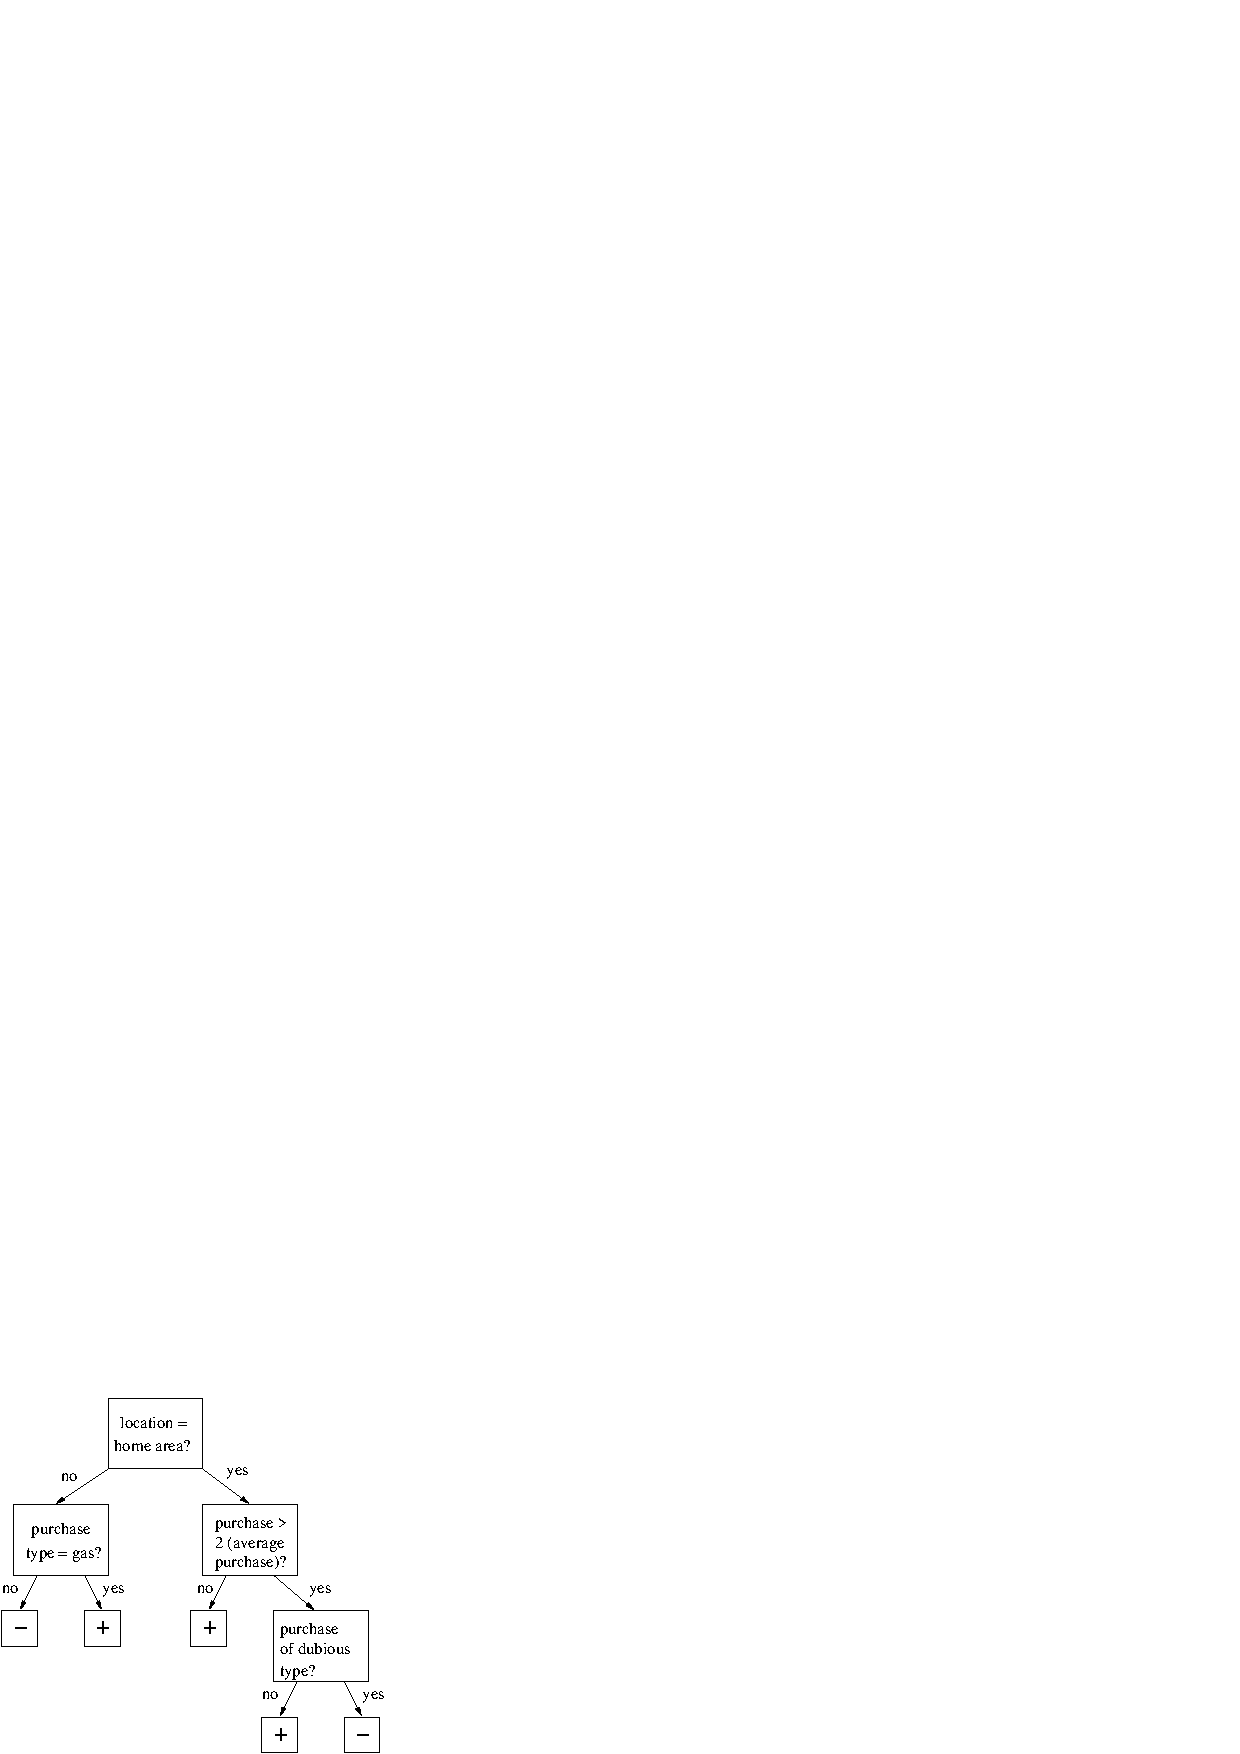
\includegraphics[width=3.5in]{figs/decision.pdf}
\end{center}

\noindent
(We assume the vectorial representation is sufficiently rich that each question can be 
answered by looking at a single coordinate of $x$.) 

How can such a tree be learned from data? The answer is, by building it top-down,
adding nodes greedily to {\it reduce uncertainty}.

\subsection{Learning a decision tree}

Suppose the training set has 10000 points, with
\begin{enumerate}
\item[] $6000$ legitimate ($+$)
\item[] $4000$ fraudulent ($-$)
\end{enumerate}
If we were allowed just one node, it would be a leaf with label ``$+$'':

\begin{center}
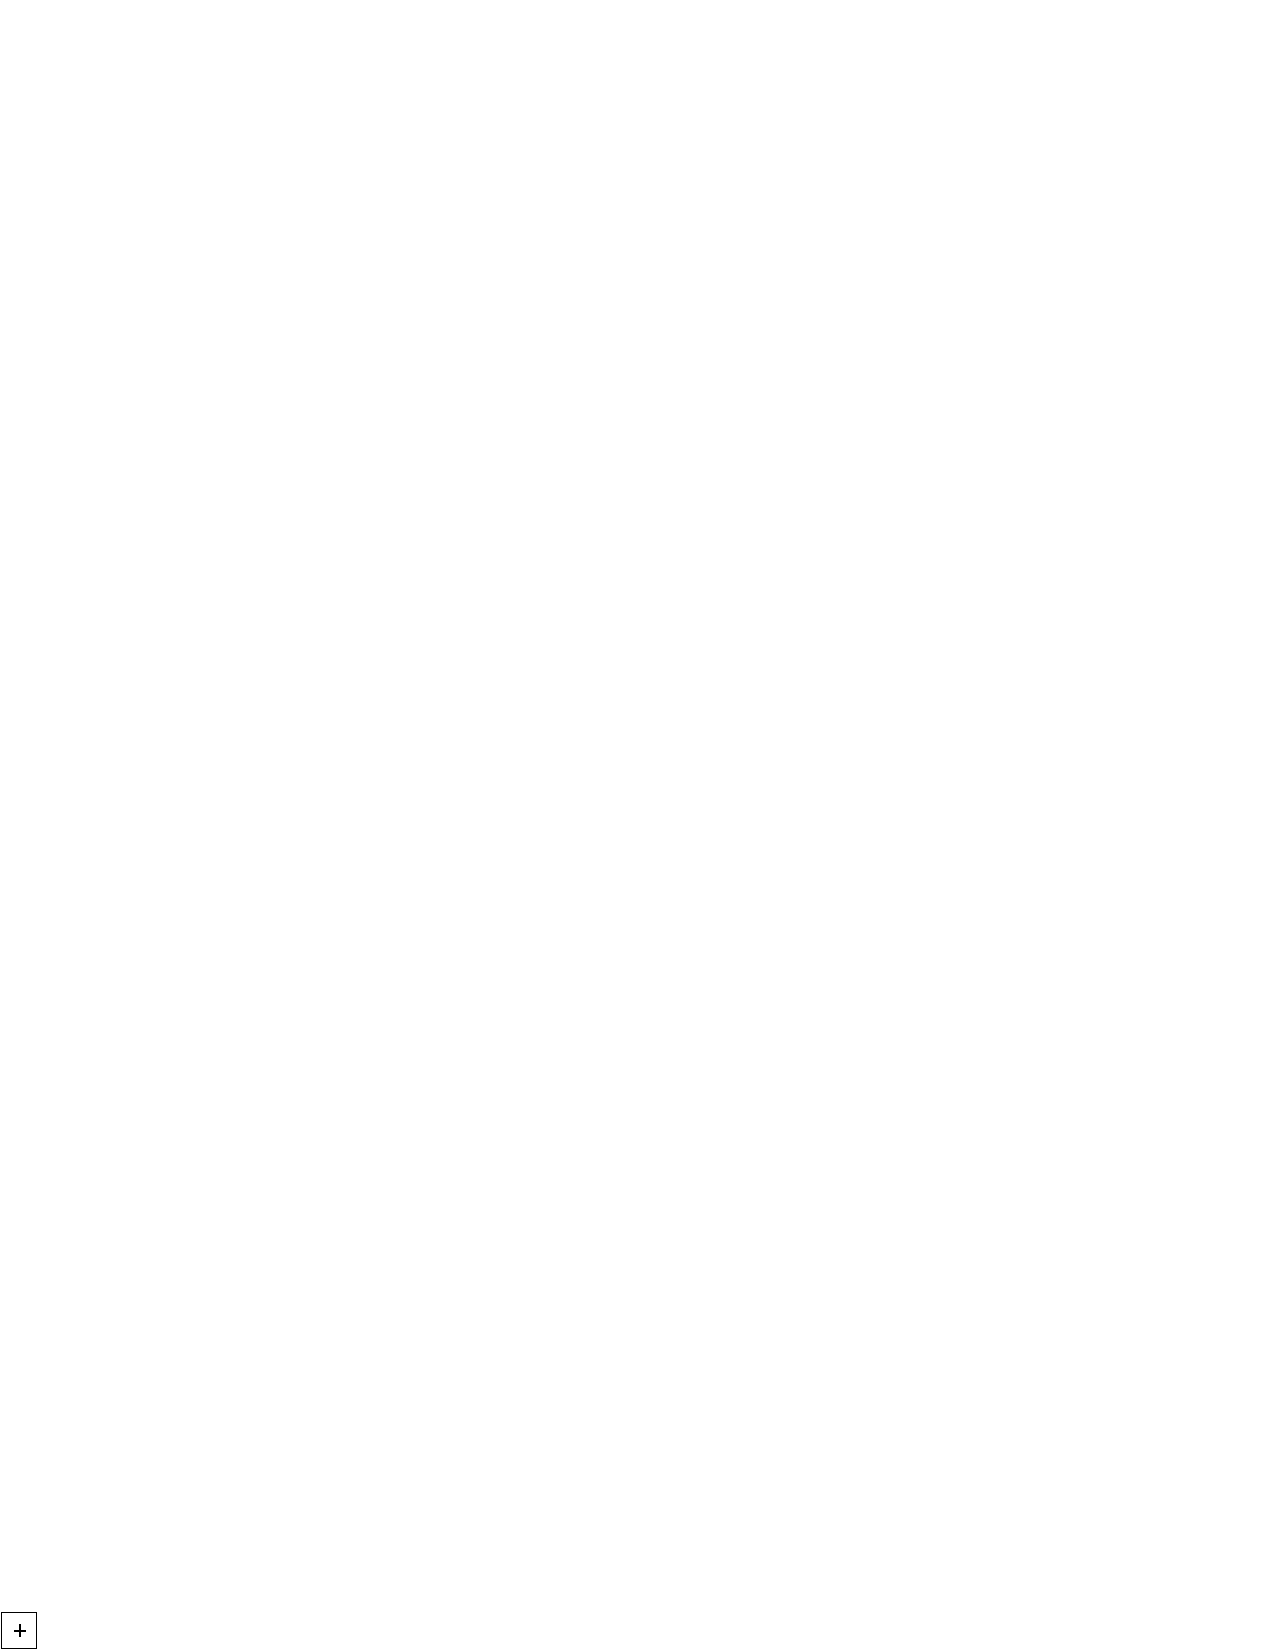
\includegraphics[width=0.3in]{figs/decision1.pdf}
\end{center}

\noindent
This has an error rate of $40\%$ on the training data.

Now suppose we were allowed just one question. For instance, we might ask whether
the location of the purchase is in the customer's home area. The answer to this 
question, yes or no, splits the training set into two subsets. Let's say the
breakdown is as follows.

\begin{center}
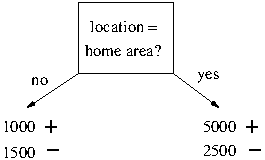
\includegraphics[width=2.5in]{figs/decision2.pdf}
\end{center}

\noindent
Then on the left leaf we'd predict ``$-$'' while on the right we'd predict
``$+$'', yielding:

\begin{center}
\includegraphics[width=2.25in]{figs/decision3.pdf}
\end{center}

A quarter of the training points end up in the left leaf, and amongst them the
error rate is $2/5$. Three-quarters of the points end up in the right leaf, and
amongst them the error rate is $1/3$. Thus the overall error rate is now
$$ \frac{1}{4} \cdot \frac{2}{5} + \frac{3}{4} \cdot \frac{1}{3} 
\ = \ \frac{7}{20},$$
or $35\%$, less than before!

So asking this particular question reduces the error rate. We should pick the
question that {\it most} reduces the error, and then recurse on the leaves. Here's
the procedure:
\begin{itemize}
\item Start with a single leaf node for all the training points.
\item Repeat:
\begin{itemize}
\item Pick a leaf that has significant error and contains quite a lot of training points.
(If there is no such leaf, halt.)
\item Split it by asking a question that maximally reduces error within the leaf.
\end{itemize}
\end{itemize}

\section{Linear classifiers}

\subsection{Document classification}

The internet brings with it a host of important {\it document classification} tasks.
For instance,
\begin{itemize}
\item Is an email message spam or not? Input: email, label: $+$ (legitimate) or $-$ (spam).
\item {\it Sentiment detection.} Is an article (such as a review) positive/favorable about 
its subject or negative/unfavorable? Input: article, label: $+$ (favorable) or $-$ 
(unfavorable).
\item Is the text on a webpage pornographic (in which case Google wouldn't want to return
it) or not? Input: text on webpage, label: $+$ (suitable for general audiences) or $-$ 
(pornographic).
\end{itemize}

As always, one approach towards solving these problems is to hand-code rules. For instance, 
given the large volume of spam that seems to involve getting money out of Nigerian bank 
accounts, a possible rule for spam might be to flag emails containing the words 
``Nigeria'' and ``bank''. But vast numbers of such rules are needed, and they are
constantly changing. It is more convenient and reliable to {\it learn} rules 
automatically from data.

\subsection{The input space $\X$ and label space $\Y$}

A document is a sequence of words, and different documents have different lengths. How can
they be represented as vectors of fixed dimension? The standard way to do so is the 
{\it bag of words} model.

Start by picking a fixed list of words, for instance, $50{,}000$ of the most common words
in English. Now represent each document as a vector $x$ with $50{,}000$ coordinates, each
associated with a particular word. That coordinate records how many times the word occurs
in the document. For example, the really short piece of text
\begin{quote}
a rose is a rose
\end{quote}
would correspond to a vector in which the coordinate for ``a'' has value 2, the
coordinate for ``is'' has value 1, the coordinate for ``rose'' has value 2,
and the remaining $49,997$ coordinates are zero.

Thus $\X = \R^{50000}$ and $\Y = \{+,-\}$. As always, we will need a training set
$(x_1, y_1), \ldots, (x_n, y_n)$, to guide our choice of classifier, as well as a 
test set on which to evaluate our final classifier.

\subsection{Linear classifiers}

Suppose the data lie in $\R^2$ instead of $\R^{50000}$. Then we can plot each training
point $x_i$ and annotate it with its label $y_i$.

\begin{center}
\includegraphics[width=2in]{figs/linear1.pdf}
\end{center}

A {\it linear classifier} $f: \R^2 \rightarrow \{+,-\}$ is simply a line with $+$ on one
side and $-$ on the other side. Future points can be classified by which side of the line
they lie on.

\begin{center}
\includegraphics[width=2in]{figs/linear2.pdf}
\end{center}

\noindent
This also works in higher dimension---that is, when $\X = \R^d$---but instead of a line
we have a $(d-1)$-dimensional hyperplane. For instance, when $d=3$ the boundary between
positive and negative is a plane.

\subsection{Learning a linear classifier}

Given a training set $(x_1, y_1), \ldots, (x_n, y_n)$, we'd like to find a linear
function $f$ that correctly classifies all the points, that is, $f(x_i) = y_i$ 
for all $i$. There are two complications, however.

First, in the example above there are infinitely many solutions: infinitely many
ways to draw a line between the positive and negative points. Which one should be
used? A popular choice is to pick the line that is most squarely in the middle
(according to a precise criterion), something like:

\begin{center}
\includegraphics[width=2in]{figs/linear3.pdf}
\end{center}

A second problem is that sometimes there is no linear classifier that gets all
the points correct:

\begin{center}
\includegraphics[width=2in]{figs/linear4.pdf}
\end{center}

\noindent
In such cases, we'd like to pick a linear function that makes the fewest mistakes 
possible (or some approximation thereof). Both these problems are handled by the
widely-used {\it support vector machine}. We won't get into the details here, but
there are plenty of software packages that will take as input a data set and 
produce a linear classifier from it.

In fact, there are further extensions that allow the boundary between the two 
classes to be nonlinear (quadratic, or cubic, or even pretty arbitrary), and 
that allow non-vector data such as DNA sequences or trees!



